\chapter{Grundlagen}

Dieses Kapitel beschreibt Grundlagen, die für das weitere Verständnis der Arbeit benötigt werden.

\section{Straßenverkehrszentrum Baden-Württemberg} % Mi

\section{Histogramm} % Mi

\section{Faltungskerne} % Mo
Faltungskerne beschreiben Filter in der Bildverarbeitung, die über die diskrete Faltung im 2-dimensionalen
Raum auf ein Bild angewendet werden.


Grundsätzlich ist die 1-dimensionale Faltung im kontinuierlichen Raum definiert durch die Integration zweier Funktionen {\em g} und {\em f} an einem Punkt {\em t}, wobei die Funktion {\em g} gespiegelt wird, also auf {\em f} gefaltet wird:

$$ (f * g)(t) = \int_{-\infty}^{\infty} f(\tau)g(t - \tau) d\tau $$

Für die Bildverarbeitung ist jedoch die Faltung im kontinuierlichen 2-dimensionalen Raum relevant.
Hierfür wird statt dem Integral, die Doppelsumme über alle Werte {\em n} gebildet (in {\em x}- und {\em y}-Richtung) und der Filter {\em k} mit dem Bild {\em I} an einem Punkt {\em (x, y)} gefaltet:

$$ I\mbox{*}(x, y) = \sum_{i=1}^{n}\sum_{j=1}^{n} I(x - i, y - j)k(i, j) $$

Hiermit wird nun eine Faltungsmatrix, bzw. ein Faltungskern auf jeden Pixel im Bild angewendet:

$$ k = \left( \begin{array}{rrr}
1 & 1 & 1 \\
1 & 1 & 1 \\
1 & 1 & 1 \\
\end{array}\right) $$

Faltungskerne sind lokale Operatoren, die die Neuberechnung eines Pixels mittels eines Teilbereichs des Bildes durchführen.
Mit solchen Filtern lassen sich Bilder beispielsweise Schärfen, Glätten. Es lassen sich jedoch auch Kanten finden oder Rauschanteile reduzieren.

\subsection{Gauß-Filter}
Der Gauß-Filter ist ein Faltungskern, welcher über eine gaußsche Glockenkurve gebildet wird.
Mit solch einem Filter lassen sich Bilder glätten und somit Rauschanteile reduzieren.
Bilder wirken dadurch weicher, bzw. verwaschen.

Ein möglicher Faltungskern sähe so aus:

$$ \frac{1}{16} \left( \begin{array}{rrr}
1 & 2 & 1 \\
2 & 4 & 2 \\
1 & 2 & 1 \\
\end{array}\right) $$

Wendet man diesen Filter auf ein Bild mit der diskreten Faltung an, erhält man dieses Ergebnis:

\begin{figure}[ht]
   \centering
     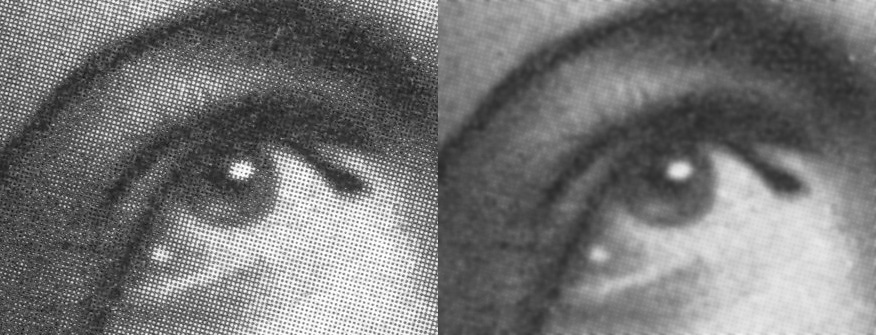
\includegraphics[width=11cm]{Bilder/Gaussian_Blur} \\
 \caption{Anwendung eines Weichzeichnungsfilters}
 \source{https://de.wikipedia.org/wiki/Datei:Halftone,_Gaussian_Blur.jpg}{10.3.2019}
 \label{fig:Blur}
\end{figure}

\subsection{Laplace-Filter}
Ein Laplace-Filter ist ein Faltungskern zur Kantendetektion innerhalb eines Bildes.
Unter einer Kante versteht man hierbei eine rasche Veränderung der Helligkeitswerte entlang einer Richtung.

Um Kanten zu finden wird ein Operator auf das Bild angewendet, welcher die zweite Ableitung bildet (Laplace-Operator). Abrupte Schwankungen der Intensitätswerte werden dadurch als Nulldurchgänge sichtbar.

Über die Faltung des Operators der Vorwärtsdiffenz {\em (1 -1)} mit sich selbst, lässt sich ein 1-dimensionaler Faltungskern der zweiten Ableitung bilden: {\em (1 -2 1)}.
Dieser Kern lässt sich transponieren, um ein Bild nicht nur in x-, sondern auch in y-Richtung abzuleiten.
Beide Kerne kombiniert ergeben den Laplace-Filter:

$$ \left( \begin{array}{rrr}
0 & 1 & 0 \\
1 & -4 & 1 \\
0 & 1 & 0 \\
\end{array}\right) $$

Wendet man diesen Filter auf ein Bild an, erhält man folgendes Ergebnis:

\begin{figure}[ht]
   \centering
     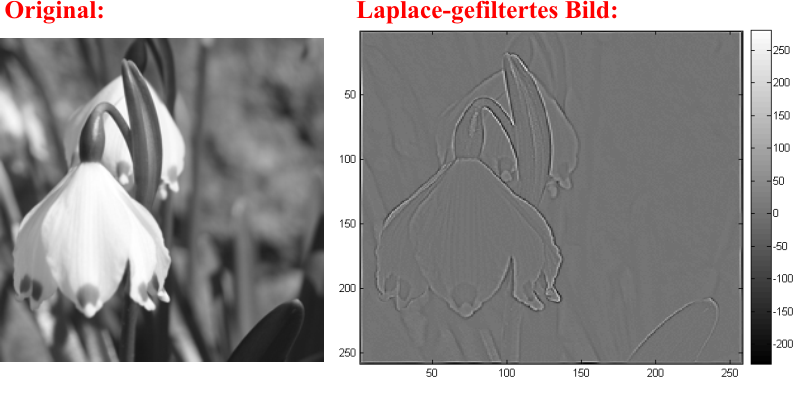
\includegraphics[width=11cm]{Bilder/Laplace} \\
 \caption{Anwendung eines Laplace-Filters}
 \source{https://de.wikipedia.org/wiki/Datei:Laplace_beispiel.png}{10.3.2019}
 \label{fig:Laplace}
\end{figure}

Aufgrund eines hohen Rauschanteils in natürlichen Bildern liefert dieser Filter jedoch nicht immer gute Resultate.

\subsection{Sobel-Operator}
Um auf natürlichen Bildern Kanten zuverlässig zu erkennen, kombiniert der Sobel-Operator die Ideen des Gauß- und Laplace-Filters.
Hierbei wird das Bild in eine Richtung über die zentrale Differenz {\em (1 0 -1)} abgeleitet, andere Richtung jedoch über einen Gauß-Filter {\em (1 2 1)} geglättet,
um Rauschanteile zu reduzieren.
Kombiniert man beide Filter miteinander, erhält man den Sobel-Operator

$$ \left( \begin{array}{rrr}
-1 & 0 & 1 \\
-2 & 0 & 2 \\
-1 & 0 & 1 \\
\end{array}\right) $$

Dadurch werden Kanten jedoch nur in eine Richtung erkannt.
Um Kanten in die jeweils andere Richtung zu erkennen, kann die Faltungsmatrix transponiert werden und ebenfalls auf
das Ausgangsbild angewendet werden.

Die beiden erhaltenen Ergebnisse können nun vereint werden, um alle Kanten innerhalb eines Bildes zu erhalten:

\begin{figure}[ht]
   \centering
     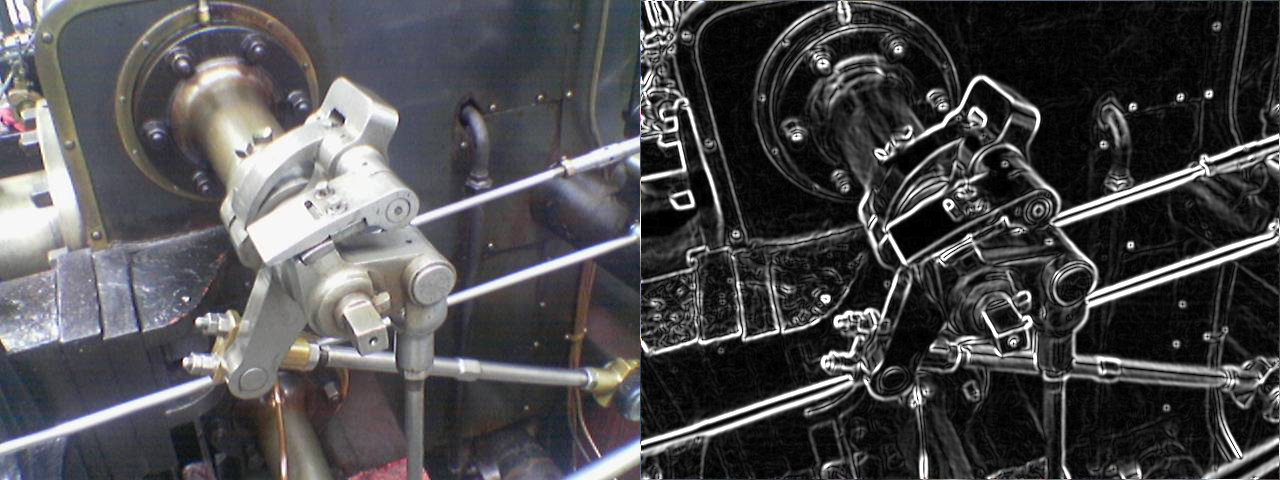
\includegraphics[width=11cm]{Bilder/Sobel} \\
 \caption{Anwendung eines Sobel-Operators}
 \source{https://en.wikipedia.org/wiki/File:Valve_sobel_(3).PNG}{10.3.2019}
 \label{fig:Sobel}
\end{figure}

\section{Canny-Edge-Detection} % Mi
\section{Otsu} % Mi
\section{Haar-Features} % Mi

\section{Morphologische Operatoren} % Mo
\subsection{Erosion}
\subsection{Dilatation}
\subsection{Closing}
\subsection{Opening}

\section{OpenCV} % Mi
